Out-of-time pileup (OOT-PU) arises when energy deposits originating from interactions in preceding bunch crossings contribute to the signal recorded in the current bunch crossing.
Since the scintillation pulse produced in ECAL crystals extends beyond the 25~ns bunch spacing, signals from multiple bunch crossings can overlap and distort the reconstructed pulse shape.
This effect degrades the timing reconstruction and introduces dependencies on both the bunch-crossing (BX) position within a filled train and the signal amplitude.

The impact of OOT-PU on the time reconstruction can be studied by examining the mean rechit time as a function of the BX position within a train of filled buckets.
Figure~\ref{cclhcplots1} shows the mean rechit time by BX for rechits reconstructed with the ratio and CC algorithms, for minimum rechit energies of 2~GeV and 20~GeV.
For this comparison, rechit times are calibrated by subtracting the mean time averaged over all BXs for rechits with energy greater than 5~GeV in the corresponding collection.

\begin{figure}[h!tbp]
\begin{center}
\resizebox{0.7\textwidth}{!}{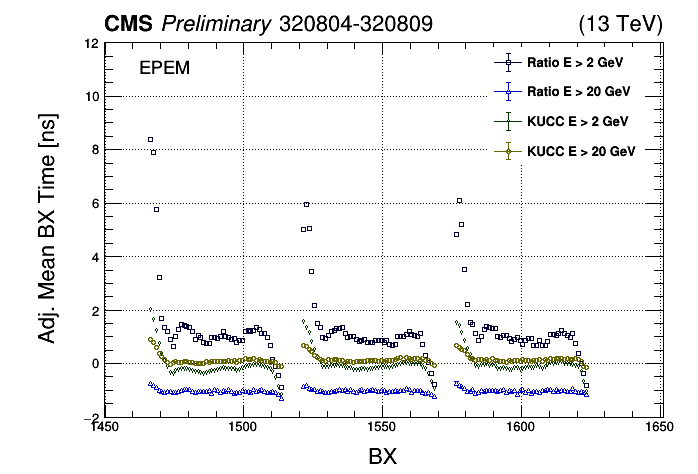
\includegraphics{fig/sec_results/tr_lhc_18A_v25_talk_30112021151421.png}}
\caption{Mean rechit time as a function of bunch-crossing position within a typical train of filled buckets, shown for the ratio and CC timing reconstructions.
Results are shown for minimum rechit energies of 2~GeV and 20~GeV.
The CC algorithm exhibits a reduced dependence on BX position and a significantly smaller energy dependence than the ratio method, demonstrating improved mitigation of OOT pileup.}
\label{cclhcplots1}
\end{center}
\end{figure}

In the leading and trailing regions of the bunch trains, the CC algorithm substantially reduces the dependence of the reconstructed time on BX position compared to the ratio algorithm.
In the central region of the trains, the separation between the 2~GeV and 20~GeV samples is significantly smaller for the CC reconstruction, indicating a markedly reduced energy dependence.
Together, these features demonstrate the improved robustness of the CC algorithm against OOT-PU effects across the full bunch train.

During the development of the CC reconstruction in Run~II, a two-tier processing strategy was employed in which rechit collections produced with both the CC and ratio algorithms were stored simultaneously.
This approach enabled a direct, event-by-event comparison of the two timing methods using identical detector conditions and reconstruction inputs.
Performance studies were carried out in both simulation and recorded data using this strategy.

The intrinsic performance of the CC algorithm was first studied in simulation by comparing its resolution to that obtained with the ratio algorithm and to the generator-level timing information derived from \texttt{pCaloHits}.
Since the reconstructed pulses used by the timing algorithms are simulated from \texttt{pCaloHits}, the resolution obtained using the generator-level time provides a reasonable estimate of the optimal achievable performance.
Figure~\ref{pc_rt_cc_comp} shows the single-crystal same readout unit (SRU) resolution as a function of effective amplitude for the ratio algorithm, the CC algorithm, and the generator-level reference.
The CC algorithm exhibits a significantly narrower resolution than the ratio method across the full amplitude range and approaches the generator-level resolution at high effective amplitudes.

\begin{figure}[h!tbp]
\begin{center}
\resizebox{0.7\textwidth}{!}{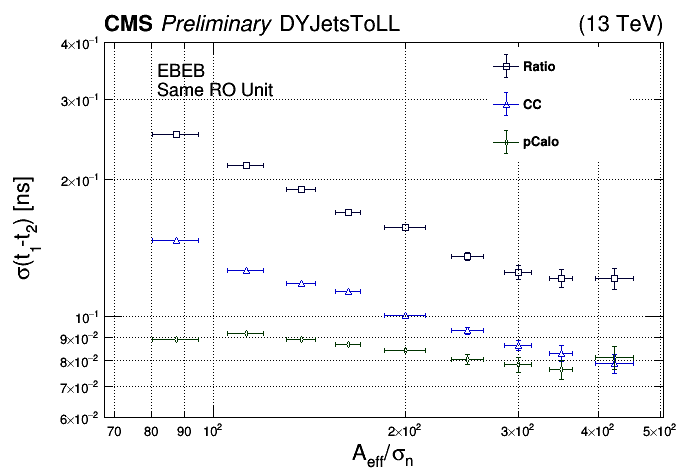
\includegraphics{fig/sec_gen/tr_mc_pc2_loc_plot_30112021153817.png}}
\caption{Single-crystal same readout unit (SRU) resolution in simulation for the ratio algorithm, the CC algorithm, and generator-level (\texttt{pCaloHit}) timing.
The CC algorithm achieves a significantly improved resolution relative to the ratio method and approaches the generator-level resolution at high effective amplitudes.}
\label{pc_rt_cc_comp}
\end{center}
\end{figure}

Figure~\ref{ccresr2} shows the same readout unit (SRU) and $Z \rightarrow e^{+}e^{-}$ object-level (ZEE) timing resolutions measured in Run~II data using the two-tier processing approach and external calibrations.
The CC algorithm improves the SRU resolution by approximately 30~ps and the ZEE resolution by approximately 35~ps relative to the ratio algorithm.

\begin{figure}[h!tbp]
\begin{center}
\resizebox{0.7\textwidth}{!}{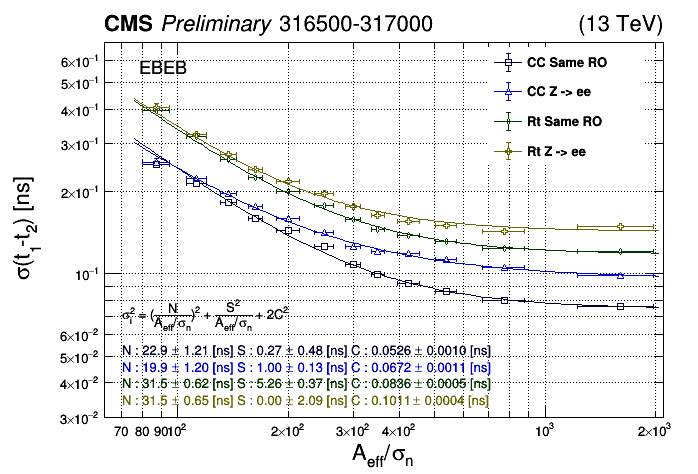
\includegraphics{fig/sec_results/tr_kucc_18As_v25_talk_30112021160215.png}}
\caption{Comparison of same readout unit (SRU) and $Z \rightarrow e^{+}e^{-}$ object-level (ZEE) timing resolutions for the ratio and CC algorithms in Run~II data, using two-tier processing and external calibrations.
The CC algorithm improves the SRU resolution by approximately 30~ps and the ZEE resolution by approximately 35~ps.}
\label{ccresr2}
\end{center}
\end{figure}

In Run~III, the CC timing algorithm was fully integrated into CMSSW and a dedicated online calibration was introduced.
Figure~\ref{ccresr3} compares the timing resolutions obtained from two independent prompt reconstructions of the same Run~III dataset, one using the ratio method and the other using the CC method as the default time reconstruction.
An improvement of approximately 80~ps in the SRU resolution is observed for the CC reconstruction.

\begin{figure}[h!tbp]
\begin{center}
\resizebox{0.7\textwidth}{!}{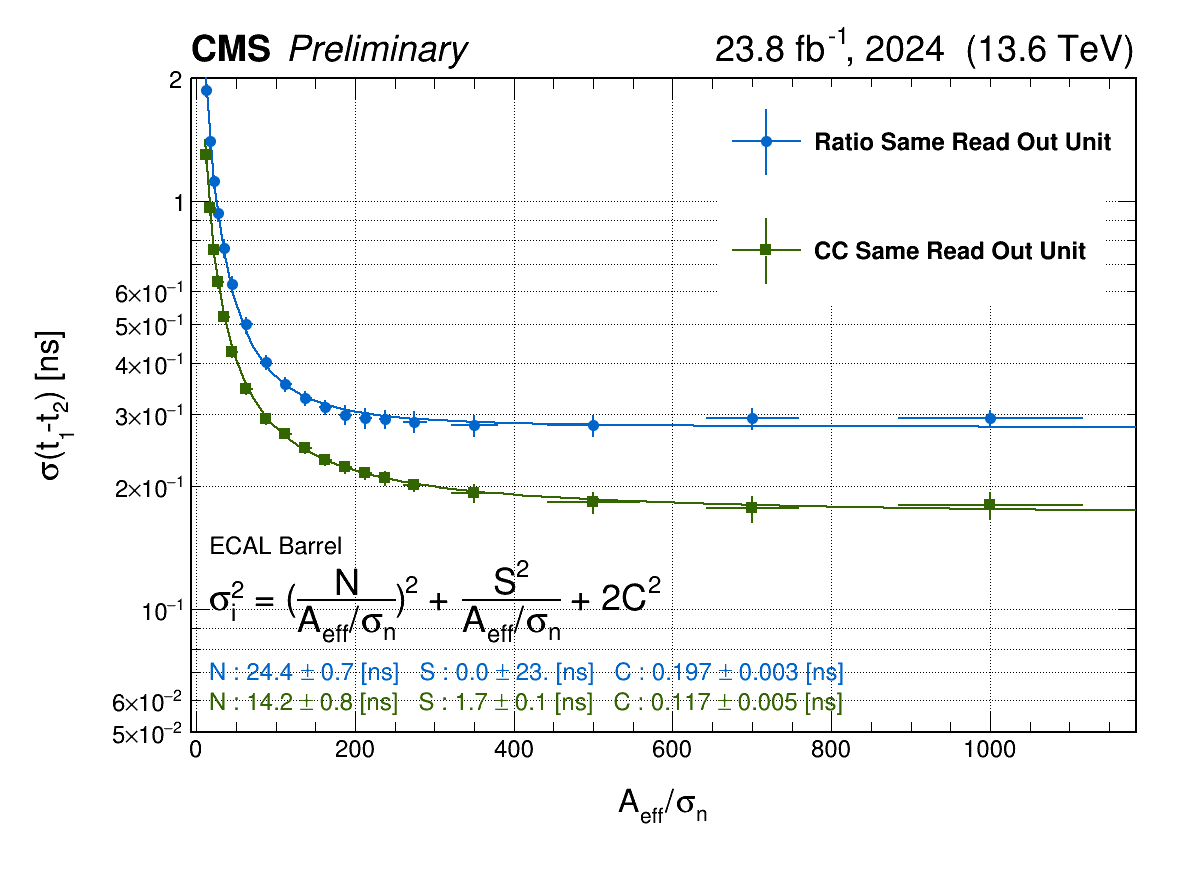
\includegraphics{fig/sec_results/tr_hl_r3_24f_v2_rtvcc_xgs_07082025170637.png}}
\caption{Comparison of same readout unit (SRU) and $Z \rightarrow e^{+}e^{-}$ object-level (ZEE) timing resolutions for the ratio and CC algorithms in Run~III.
The results are obtained from two independent prompt reconstructions of the same dataset.
An improvement of approximately 80~ps in the SRU resolution is observed for the CC algorithm.}
\label{ccresr3}
\end{center}
\end{figure}

A particularly informative comparison is provided by data collected during the 2024F data-taking period.
In this era, two independent prompt reconstructions of the same dataset were produced using official online CMS calibrations, differing only in the choice of the default ECAL timing reconstruction algorithm.
One reconstruction employed the ratio-based timing method, while the other used the CC algorithm as the default time reconstruction.
This configuration enables a direct comparison of the two timing algorithms under identical detector conditions, calibration strategies, and pileup environments, without relying on external or offline reprocessing.

The timing resolutions obtained in the 2024F data-taking period are shown in Fig.~\ref{ccresr2024F}.
A clear improvement is observed when the CC algorithm is used as the default ECAL timing reconstruction in prompt reconstruction.
Relative to the ratio-based method, the CC algorithm achieves a significantly improved same readout unit (SRU) resolution, together with a corresponding improvement in the $Z \rightarrow e^{+}e^{-}$ object-level (ZEE) timing resolution.
These results demonstrate that the performance gains observed in earlier two-tier studies persist when the CC algorithm is deployed as the default timing reconstruction within the full CMS prompt reconstruction chain using official online calibrations.
In the 2024F era, the CC reconstruction improves the SRU resolution by approximately XX~ps and the ZEE resolution by approximately YY~ps relative to the ratio-based reconstruction.

% added plots
\begin{figure}[h!tbp]
\begin{center}
\resizebox{0.7\textwidth}{!}{\includegraphics{fig/sec_results/tr_rtvcc_2024F_prompt_placeholder.png} }
\caption{Comparison of same readout unit (SRU) and $Z \rightarrow e^{+}e^{-}$ object-level (ZEE) timing resolutions obtained during prompt reconstruction in the 2024F data-taking period.
Two independent prompt reconstructions of the same dataset are compared, one using the ratio-based timing algorithm and the other using the CC algorithm as the default ECAL time reconstruction, both with official online CMS calibrations.
The CC algorithm exhibits improved SRU and ZEE timing resolutions relative to the ratio-based reconstruction.}
\label{ccresr2024F}
\end{center}
\end{figure}

Figure~\ref{ccresr4} shows the timing performance of the CC algorithm during the 2025 Run~III data-taking period, in which the CC reconstruction was used exclusively as the default ECAL timing algorithm for prompt reconstruction, together with its corresponding online calibration.
In this configuration, the CC algorithm achieves an SRU resolution of approximately 135~ps and a ZEE resolution of approximately 180~ps in prompt reconstruction.
Comparing the ZEE resolution achieved with the CC algorithm to the SRU resolution obtained with the ratio algorithm in Run~III demonstrates that the CC reconstruction substantially mitigates the impact of OOT-PU on analysis-relevant timing performance.
These improvements directly enhance the sensitivity of analyses relying on ECAL timing, particularly in high-pileup environments.

\begin{figure}[h!tbp]
\begin{center}
\resizebox{0.7\textwidth}{!}{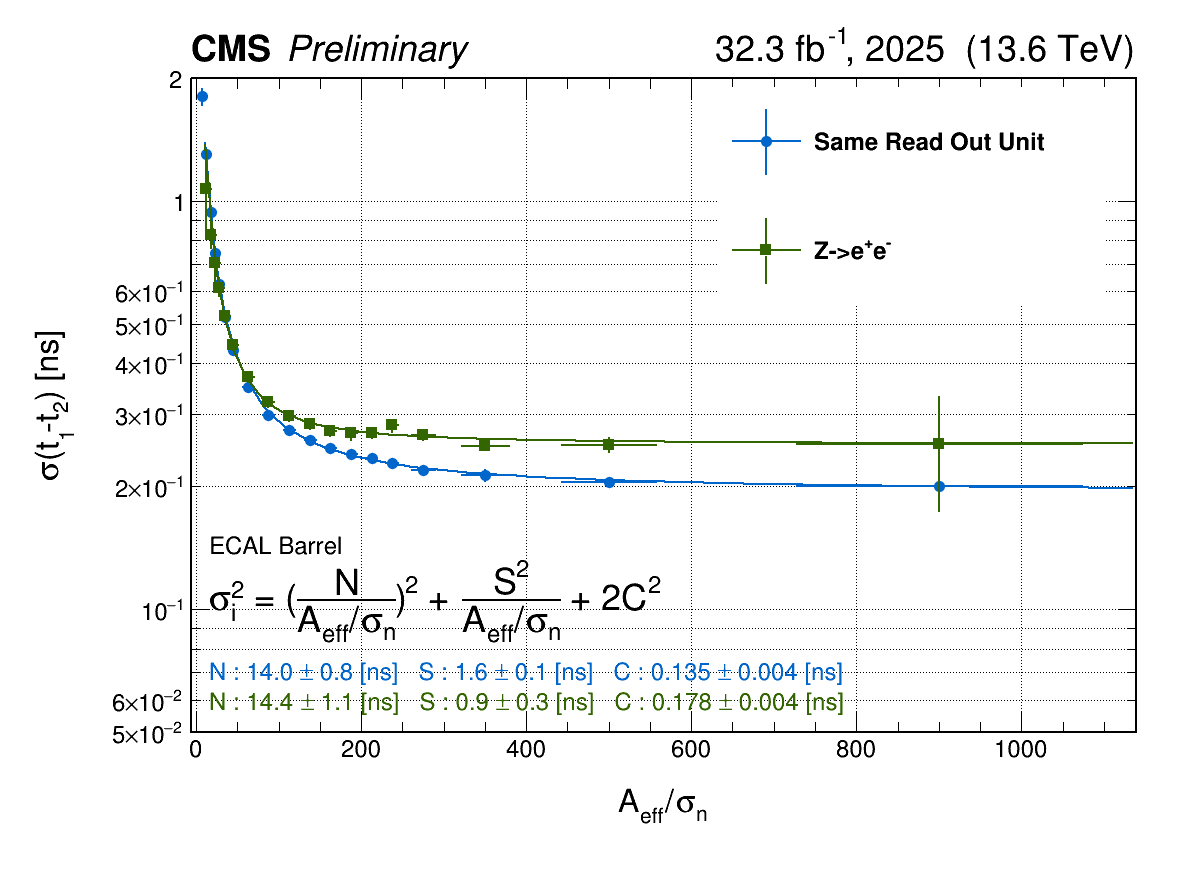
\includegraphics{fig/sec_results/tr_hl_r3_25c2_08082025165318.png}}
\caption{Same readout unit (SRU) and $Z \rightarrow e^{+}e^{-}$ object-level (ZEE) timing resolutions obtained with the CC algorithm during prompt reconstruction in Run~III (2025).
The CC algorithm, together with a dedicated online calibration, achieves an SRU resolution of approximately 135~ps and a ZEE resolution of approximately 180~ps.}
\label{ccresr4}
\end{center}
\end{figure}
